% !TEX root = ../thesis.tex

\chapter{Training der Machine-Learning-Klassifikatoren}
\label{training}

Dieses Kapitel gibt einen Überblick über das Training der Machine-Learning-Klassifikatoren. Dazu werden zunächst die Auswahl des verwendeten Werkzeugs und die Auswahl der Klassifikationsalgorithmen erläutert. Anschließend findet eine Darlegung des Trainingsprozesses statt. Es werden somit die Arbeitsschritte erläutert, welche durchgeführt wurden, um das zweite Forschungsziel \glqq Identifikation und Training einer Auswahl von relevanten Machine-Learning-Klassifikatoren basierend auf dem Datenset\grqq{} abzuschließen. Darüber hinaus werden die folgenden Forschungsfragen beantwortet:
\vspace{-\topsep}
\begin{itemize}
\setlength{\itemsep}{-2pt}
\item RQ2: Welche Machine-Learning-Klassifikatoren kommen für die gegebene Aufgabe in
Frage?
\item RQ3c: Wie lassen sich die Klassifikatoren mit einer klassischen Vorhersagetechnik, die keine Features nutzt, vergleichen?
\end{itemize}
\smallskip
\hrule

\section{Auswahl des Werkzeugs und der Klassifikationsalgorithmen}

Zur Anwendung als Machine-Learning-Werkzeug kommt die WEKA-Workbench\footnote{\href{https://www.cs.waikato.ac.nz/ml/weka/}{https://www.cs.waikato.ac.nz/ml/weka/}}. Im Rahmen der strukturierten Literaturanalyse zu Beginn der Erarbeitung der Masterarbeit, erwies sich dieses Werkzeug aufgrund zahlreicher Zitierungen in wissenschaftlichen Arbeiten (zum Beispiel in \cite{Hammouri2018,Ratzinger2008}) als geeignet für die zugrundeliegende Aufgabe. Darunter befinden sich auch die wissenschaftlichen Arbeiten, die in \hyperref[ml-background]{Abschnitt 2.3} als Beispiele zum Thema der Fehlervorhersage mittels Machine Learning vorgestellt wurden und Grundlagen für diese Ausarbeitung darstellen \cite{Moser2008,Queiroz2016}. Die WEKA-Workbench (WEKA als Akronym für \textbf{W}aikato \textbf{E}nvironment for \textbf{K}nowledge \textbf{A}nalysis) wurde an der University of Waikato in Neuseeland entwickelt und bietet eine große Kollektion an Machine-Learning-Algorithmen und Preprocessing-Tools zur Verwendung innerhalb einer grafischen Benutzeroberfläche \cite{Weka2016}. Es existieren zudem Schnittstellen für die Programmiersprache Java \cite{Weka2016}.

Eine Übersicht über die ausgewählten Klassifikationsalgorithmen befindet sich in \autoref{tab:classifiers}. Diese umfasst auch die Abkürzungen der Klassifikatoren, die im weiteren Verlauf der Arbeit verwendet werden. Ausführliche Erläuterungen zu den Algorithmen wurden bereits zuvor in \hyperref[algorithms]{Abschnitt 2.1} gegeben.

\begin{table}[ht]
\centering
\caption{Zum Training verwendete Klassifikationsalgorithmen}
\label{tab:classifiers}
\resizebox{\linewidth}{!}{%
\begin{tabular}{|>{\hspace{0pt}}p{0.692\linewidth}|>{\hspace{0pt}}p{0.304\linewidth}|} 
\hline
\textbf{Algorithmus}        & \textbf{Abkürzung}  \\ 
\hline
J48 Decision Trees          & J48                 \\ 
\hline
k-Nearest-Neighbors         & KNN                 \\ 
\hline
logistische Regression      & LR                  \\ 
\hline
Na\"{\i}ve Bayes                 & NB                  \\ 
\hline
künstliche neuronale Netze  & NN                  \\ 
\hline
Random Forest               & RF                  \\ 
\hline
Stochastic Gradient Descent & SGD                 \\ 
\hline
Support Vector Machines     & SVM                 \\
\hline
\end{tabular}
}
\end{table}

Alle zuvor vorgestellten Klassifikationsalgorithmen sind bereits im Werkzeug WEKA integriert. Es erhält als Eingabe die finalen Datensets in einem proprietären Dateiformat, deren Erstellung im \hyperref[dataset-creation]{vorherigen Kapitel} erläutert wurde. Die 13 berechneten Metriken bilden dabei die Attribute, wohingegen die Zielklasse durch die Label \glqq defekt\grqq{} und \glqq fehlerfrei\grqq{} abgebildet wird.

\fbox{\parbox{\linewidth}{RQ2: WELCHE MACHINE-LEARNING-KLASSIFIKATOREN KOMMEN FÜR DIE GEGEBENE AUFGABE IN FRAGE?\medskip\\
Es werden acht verschiedene Klassifikationsalgorithmen zur Anwendung kommen, deren Hauptkriterium für die Auswahl die vorherige Verwendung im Rahmen der wissenschaftlichen Literatur war \cite{Son2019}. Die Algorithmen lauten: J48, KNN, LR, NB, NN, RF, SGD, SVM. Als Werkzeug für die Durchführung des Trainings der Klassifikatoren kommt der WEKA Workbench \cite{Weka2016} zum Einsatz.}}

\section{Trainingsprozess der Klassifikatoren}

Der Trainingsprozess der Klassifikatoren erfolgte innerhalb der grafischen Benutzeroberfläche von WEKA. Vor dem Training wurden die Split-Ratios für die Aufteilung der Datensets in Trainingsdaten und Testdaten festgelegt. Sie wurde für jedes der verwendeten Softwareprojekte individuell festgelegt und basiert auf der Anzahl der jeweils vorhandenen Releases. Dabei wurde jedoch stets darauf geachtet, dass die üblich verwendeten Split-Ratios von $80:20$ und $75:25$ sowie $70:30$ angenähert wurden. Die Größenordnungen der Trainingsdaten reichen von $67\%$ bis $80\%$ der Datenpunkte der Datensets. Die früheren Releases wurden den Trainingsdaten zugeordnet. Die Trainingsdaten enthalten die Datenpunkte der späteren Releases. Eine Übersicht der Aufteilung in Trainings- und Testdaten je Softwareprojekt ist in \autoref{fig:splits} dargestellt. Die daraus resultierten Split-Ratios für die gesamten Datensets lauten: $69:31$ (featurebasiertes Datenset) und $71:29$ (\glqq einfache\grqq{} und erweiterte dateibasierte Datenset).

\begin{figure}[ht]
  \centering
  \subfloat[][Blender\\Split-Ratio: $73:27$]{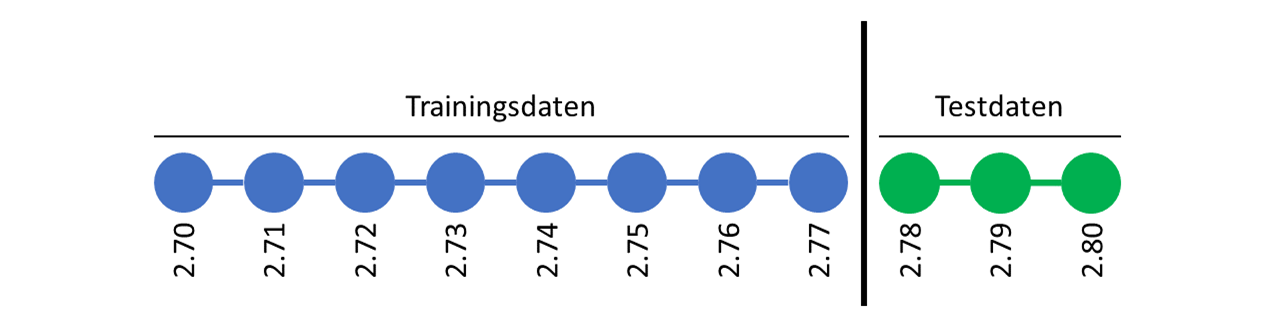
\includegraphics[width=0.5\linewidth]{images/release_blender}}
  \subfloat[][Busybox\\Split-Ratio: $71:29$]{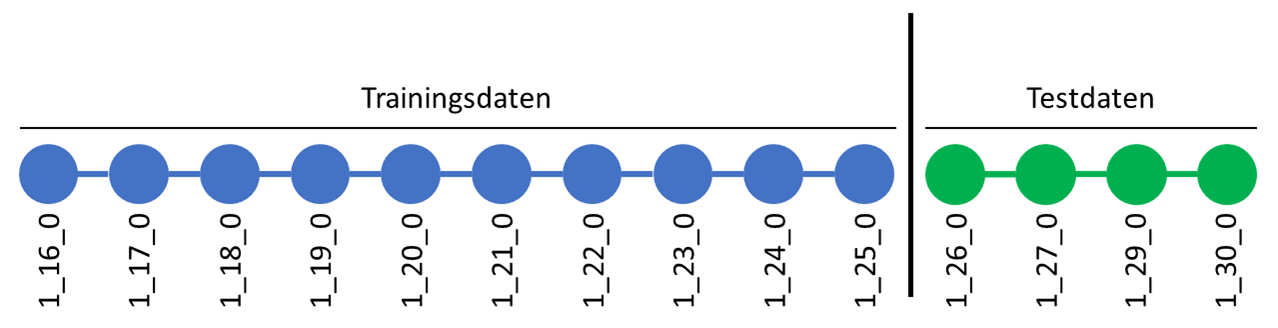
\includegraphics[width=0.5\linewidth]{images/release_busybox}}
  \qquad
  \subfloat[][Emacs\\Split-Ratio: $71:29$]{
\includegraphics[width=0.5\linewidth]{images/release_emacs}}
  \subfloat[][GIMP\\Split-Ratio: $71:29$]{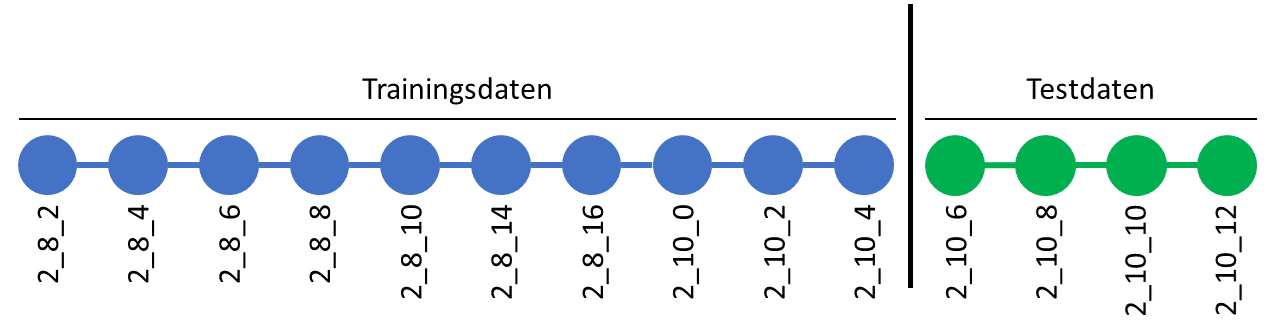
\includegraphics[width=0.5\linewidth]{images/release_gimp}}
  \qquad
  \subfloat[][Gnumeric\\Split-Ratio: $75:25$]{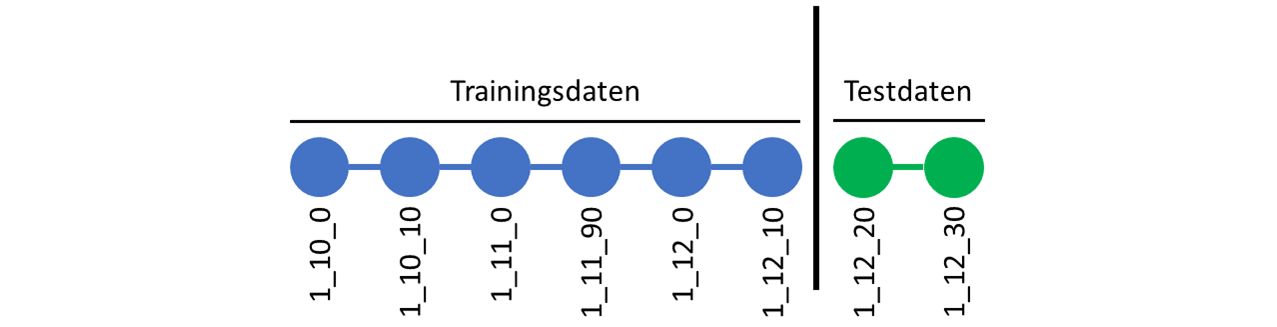
\includegraphics[width=0.5\linewidth]{images/release_gnumeric}}  
  \subfloat[][gnuplot\\Split-Ratio: $80:20$]{
\includegraphics[width=0.5\linewidth]{images/release_gnuplot}}
  \qquad
  \subfloat[][Irssi\\Split-Ratio: $71:29$]{
\includegraphics[width=0.5\linewidth]{images/release_irssi}}
  \subfloat[][libxml2\\Split-Ratio: $80:20$]{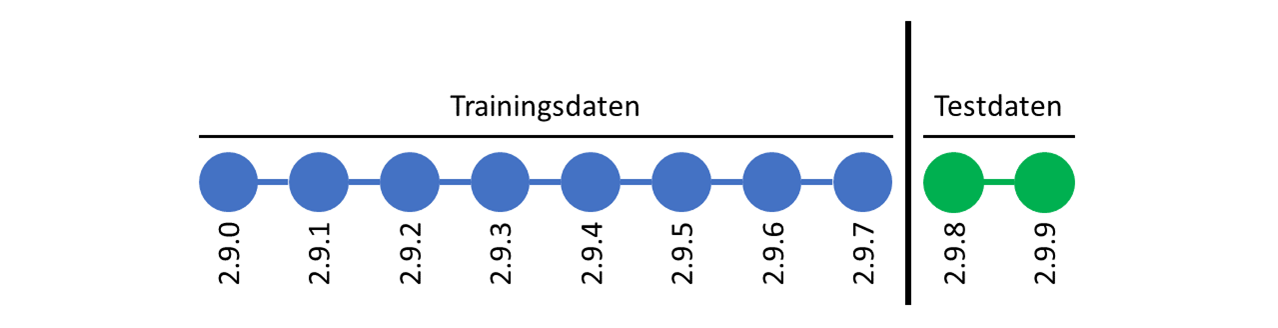
\includegraphics[width=0.5\linewidth]{images/release_libxml2}}
  \qquad
  \subfloat[][lighttpd\\Split-Ratio: $67:33$]{
\includegraphics[width=0.5\linewidth]{images/release_lighttpd}}
  \subfloat[][MPSolve\\Split-Ratio: $75:25$]{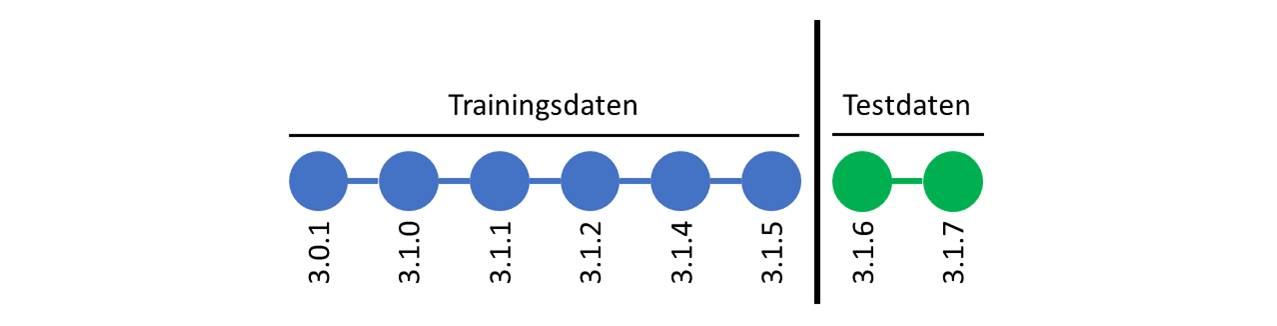
\includegraphics[width=0.5\linewidth]{images/release_mpsolve}}
  \qquad
  \subfloat[][Parrot\\Split-Ratio: $71:29$]{
\includegraphics[width=0.5\linewidth]{images/release_parrot}}
  \subfloat[][Vim\\Split-Ratio: $71:29$]{
\includegraphics[width=0.5\linewidth]{images/release_vim}}
  \caption{Übersicht der Aufteilung in Trainings- und Testdaten\label{fig:splits}}
\end{figure}

Das Training der Klassifikatoren in WEKA erfolgte für jeden Klassifikationsalgorithmus mit den jeweiligen Standardeinstellungen. Lediglich für die Algorithmen NN und RF wurden weitere Konfigurationen vorgenommen. Für den RF-Algorithmus wurde eine Instanzanzahl von 200 festgelegt. Dies bedeutet, dass gleichzeitig 200 Entscheidungsbäume parallel Verarbeitungen durchführen. Es gibt keine eindeutigen Empfehlungen, wie viele Instanzen gewählt werden sollten. Der ausgewählte Wert von 200 wurde somit unter Berücksichtigung des Umfangs der Datensets sowie der hohen Anzahl an Attributen eigenständig festgelegt. Für den NN-Algorithmus wurde eine eigenständig festgelegte Hidden-Layer-Struktur von (\texttt{(13,13,13}) gewählt. Dies bedeutet, dass das künstliche neuronale Netz drei Hidden-Layer-Schichten à 13 Hidden-Layer-Neuronen besitzt. Dies ermöglicht ihnen, die große Anzahl an Attributen effizienter zu verarbeiten. Darüber hinaus wurden keine Validierungsdaten erzeugt, da es nicht vorgesehen ist, eine Attributsauswahl durchzuführen. Die sogenannte \glqq Hyperparameteroptimierung\grqq{}, also die Anpassung verschiedener einstellbarer Parameter der Klassifikatoren zur Optimierung hinsichtlich der Verbesserung eines Wertes einer Evaluationsmetrik, erfolgt automatisch von WEKA unter Betrachtung der Accuracy.

\label{smote}
Eine Analyse des Trainingsprozesses zeigte zudem, dass die dateibasierten Datensets hinsichtlich der Zielklasse stark unbalanciert sind. Mit einem Wert von etwa $97\%$ existieren weitaus mehr Einträge, die dem Label \glqq fehlerfrei\grqq{} zugeordnet sind. Balanciertheit, also ein ausgeglichenes Verhältnis ($50:50$ ist im binären Fall nicht zwingend notwendig) innerhalb der Zielklassen, ist jedoch eine Voraussetzung für das korrekte Training der meisten Klassifikatoren. Eine Nichtbeachtung dieses Problems kann zu einer irreführenden Accuracy führen, da die meisten Datenpunkte korrekt der überrepräsentierten Klasse zugeordnet werden. Dies stellt ein grundsätzliches Problem der Accuracy-Metrik dar und überträgt sich auf die Ergebnisse der Vorhersageperformanz der Anwendung der Testdaten sowie auf die Ergebnisse von Vorhersagen unbekannter Daten. Eine übliche Herangehensweise zur Lösung dieses Problems besteht darin, zusätzliche Datenpunkte der unterrepräsentierten Klasse synthetisch zu erzeugen und dadurch ein Oversampling dieser Klasse zu erreichen. Im Rahmen der Arbeit wurde der auf dieser Idee basierende SMOTE-Algorithmus (\textbf{S}ynthetic \textbf{M}inority \textbf{O}versampling \textbf{Te}chnique, \cite{Chawla2002}) auf die datenbasierten Datenset angewandt. Anhand von nächste-Nachbarn-Berechnungen auf Basis der Euklidischen Distanz zwischen den Attributwerten der einzelnen Datenpunkte der Datensets, werden neue synthetische Datenpunkte hinzugefügt (Oversampling), sodass sich die Anzahl der Datenpunkte der relevanten Klasse erhöht \cite{Chawla2002}. Im hier durchgeführten Fall wurde der Prozentsatz für die Generierung der synthetischen Datenpunkte auf 2000 festgelegt, sodass für jeden vorhandenen Datenpunkt der unterrepräsentierten Klasse 20 zusätzliche synthetische Datenpunkte erzeugt wurden. So konnte der Anteil der Datenpunkte mit dem Label \glqq fehlerhaft\grqq{} auf etwa $41\%$ erhöht werden. Dies stellt eine ausreichende Balance zwischen den Datenpunkten dar. Gleichzeitig wuchs die Anzahl der Datenpunkte der Trainingsdaten um etwa $60\%$. Angewendet wurde der Algorithmus nur auf die Trainingsdaten \cite{Chawla2002}. Eine Anwendung auf die Testdaten ist nicht vorgesehen, damit die \glqq ground truth\grqq{} nicht verzerrt beziehungsweise verfälscht wird. Infolge dessen änderten sich zudem die Kennzahlen der dateibasierten Datensets. Diese sind in \autoref{tab:dataset-numbers-new} dargestellt.

\begin{table}[ht]
\centering
\caption{Kennzahlen der Datensets}
\label{tab:dataset-numbers-new}
\resizebox{\linewidth}{!}{%
\begin{tabular}{|>{\hspace{0pt}}p{0.283\linewidth}|>{\RaggedLeft\hspace{0pt}}p{0.175\linewidth}|>{\RaggedLeft\hspace{0pt}}p{0.177\linewidth}|>{\RaggedLeft\hspace{0pt}}p{0.175\linewidth}|>{\RaggedLeft\hspace{0pt}}p{0.179\linewidth}|} 
\hline
\multirow{2}{*}{}       & \multicolumn{2}{>{\Centering\hspace{0pt}}p{0.352\linewidth}|}{ \textbf{\glqq einfaches\grqq{} 
dateibasiertes Datenset}} & \multicolumn{2}{>{\Centering\hspace{0pt}}p{0.354\linewidth}|}{\begin{tabular}[c]{@{}c@{}}\textbf{erweitertes dateibasiertes Datenset}\end{tabular}}  \\ 
\cline{2-5}
                        & \textbf{vorher} & \textbf{nachher}                                                                        & \textbf{vorher} & \textbf{nachher}                                                                                                                             \\ 
\hline
Anzahl Attribute        & $17$ + Label      & $17$ + Label                                                                              & $28$ + Label      & $28$ + Label                                                                                                                                   \\ 
\hline
Anzahl Datenpunkte       & $76.986$          & $111.706$                                                                                 & $76.986$          & $112.706$                                                                                                                                      \\ 
\hline
~ ~ ~- davon defekt     & $1.899$           & $37.619$                                                                                  & $1.899$           & $37.619$                                                                                                                                       \\ 
\hline
~ ~ ~- davon fehlerfrei & $75.087$          & $75.087$                                                                                  & $75.087$          & $75.087$                                                                                                                                       \\ 
\hline
~ ~ ~- davon \glqq unique\grqq   & $52.564$          & $86.155$                                                                                  & $52.783$          & $86.381$                                                                                                                                       \\ 
\hline
Gesamt-Split-Ratio      & $71:29$           & $81:19$                                                                                   & $71:29$           & $81:19$                                                                                                                                        \\
\hline
\end{tabular}
}
\end{table}

Die Ergebnisse, die mithilfe der Testdaten erzielt wurden und die Performanz der einzelnen Klassifikatoren widerspiegeln, werden im folgenden Kapitel im Rahmen der Evaluation vorgestellt.

\cleardoublepage


%\begin{figure}[t]
%    \centering
%    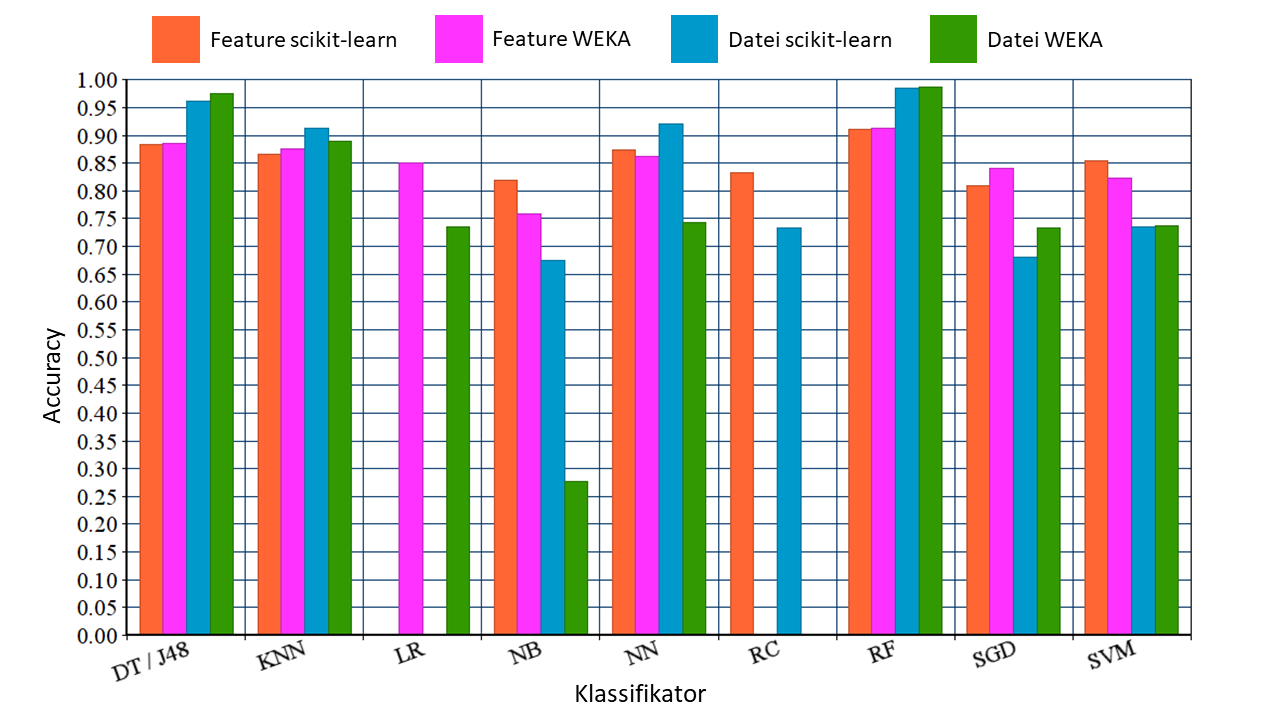
\includegraphics[width=\textwidth]{images/Vergleich1}
%    \caption{Vergleich der Klassifikatoren und Werkzeuge im Hinblick auf ihre Accuracies\label{fig:vergl1}}
%\end{figure}
%
%Zur Auswahl der effektivsten Kombination der Attribute je Klassifikator wurde auf die von scikit-learn und WEKA bereitgestellten Werkzeuge zurückgegriffen. Sowohl scikit-learn als auch WEKA konnten nicht für jeden Klassifikator der beiden Datensets Kombinationen ausgeben. Dies bedingt entweder die Funktionsweise des Klassifikationsalgorithmus, die fehlende Unterstützung der Werkzeuge für einen bestimmten Klassifikator oder eine endlose Durchführung der Ermittlung der Kombination. Eine Übersicht der Konfiguration je Klassifikator des featurebasierten Datensets ist in \autoref{tab:configs_feat} dargestellt. Die Übersicht für das dateibasierte Datenset befindet sich in \autoref{tab:configs_file}.
%
%\begin{table}[t]
%\centering
%\caption{Übersicht der Konfigurationen des featurebasierten Datensets}
%\label{tab:configs_feat}
%\resizebox{\linewidth}{!}{%
%\begin{tabular}{|l|l|l|} 
%\hline
% \textbf{Klassifikator}  & \textbf{Konfiguration scikit-learn}                                                                                                                                                                                                       & \textbf{Konfiguration WEKA}                                                                                                                                                                          \\ 
%\hline
%DT / J48                 & \begin{tabular}[c]{@{}l@{}}\begin{tabular}{@{\labelitemi\hspace{\dimexpr\labelsep+0.5\tabcolsep}}l}max\_features = \glqq sqrt\grqq\\Split-Ratio: 85:15\\Features: alle außer COMM, DDEV, MODD\end{tabular}\end{tabular}                            & \begin{tabular}[c]{@{}l@{}}\begin{tabular}{@{\labelitemi\hspace{\dimexpr\labelsep+0.5\tabcolsep}}l}Split-Ratio: 70:30\\Features: alle außer DDEV, OEXP, MODS, REML\end{tabular}\end{tabular}         \\ 
%\hline
%KNN                      & \begin{tabular}[c]{@{}l@{}}\begin{tabular}{@{\labelitemi\hspace{\dimexpr\labelsep+0.5\tabcolsep}}l}k = 1\\Split-Ratio: 75:25 \end{tabular}\end{tabular}                                                                                   & \begin{tabular}[c]{@{}l@{}}\begin{tabular}{@{\labelitemi\hspace{\dimexpr\labelsep+0.5\tabcolsep}}l}k = 1\\Split-Ratio: 65:35\end{tabular}\end{tabular}                                               \\ 
%\hline
%LR                       &                                                                                                                                                                                                                                           & \begin{tabular}{@{\labelitemi\hspace{\dimexpr\labelsep+0.5\tabcolsep}}l}Split-Ratio: 65:35\end{tabular}                                                                                              \\ 
%\hline
%NB                       & \begin{tabular}[c]{@{}l@{}}\begin{tabular}{@{\labelitemi\hspace{\dimexpr\labelsep+0.5\tabcolsep}}l}Multinomial-NB\\Split-Ratio: 75:25 \end{tabular}\end{tabular}                                                                          & \begin{tabular}[c]{@{}l@{}}\begin{tabular}{@{\labelitemi\hspace{\dimexpr\labelsep+0.5\tabcolsep}}l}Split-Ratio: 70:30\\Features: COMM,ADEV, EXP, OEXP, ADDL\end{tabular}\end{tabular}                \\ 
%\hline
%NN                       & \begin{tabular}[c]{@{}l@{}}\begin{tabular}{@{\labelitemi\hspace{\dimexpr\labelsep+0.5\tabcolsep}}l}hidden\_layer\_sizes = (13,13,13)\\StandardScaler\\max\_iter = 500\\Split-Ratio: 85:15\end{tabular}\end{tabular}                       & \begin{tabular}[c]{@{}l@{}}\begin{tabular}{@{\labelitemi\hspace{\dimexpr\labelsep+0.5\tabcolsep}}l}Hidden-Layer = (13,13,13)\\Split-Ratio: 80:20\end{tabular}\end{tabular}                           \\ 
%\hline
%RC                       & \begin{tabular}[c]{@{}l@{}}\begin{tabular}{@{\labelitemi\hspace{\dimexpr\labelsep+0.5\tabcolsep}}l}StandardScaler\\Split-Ratio: 75:25\\Features: alle außer REML\end{tabular}\end{tabular}                                                &                                                                                                                                                                                                      \\ 
%\hline
%RF                       & \begin{tabular}[c]{@{}l@{}}\begin{tabular}{@{\labelitemi\hspace{\dimexpr\labelsep+0.5\tabcolsep}}l}n\_estimators = 200\\max\_features = \glqq sqrt\grqq\\Split-Ratio: 75:25\\Features: alle außer COMM, DDEV, MODD, REML\end{tabular}\end{tabular} & \begin{tabular}[c]{@{}l@{}}\begin{tabular}{@{\labelitemi\hspace{\dimexpr\labelsep+0.5\tabcolsep}}l}Iterationen: 200\\Split-Ratio: 80:20\\Features: alle außer ADEV, OEXP \end{tabular}\end{tabular}  \\ 
%\hline
%SGD                      & \begin{tabular}[c]{@{}l@{}}\begin{tabular}{@{\labelitemi\hspace{\dimexpr\labelsep+0.5\tabcolsep}}l}loss = „log“\\penality = „elasticnet“\\Split-Ratio: 70:30\\Features: EXP, OEXP, ADDL, REML\end{tabular}\end{tabular}                   & \begin{tabular}[c]{@{}l@{}}\begin{tabular}{@{\labelitemi\hspace{\dimexpr\labelsep+0.5\tabcolsep}}l}Split-Ratio: 70:30\\Features: alle außer REML \end{tabular}\end{tabular}                          \\ 
%\hline
%SVM                      & \begin{tabular}[c]{@{}l@{}}\begin{tabular}{@{\labelitemi\hspace{\dimexpr\labelsep+0.5\tabcolsep}}l}LinearSVC\\max\_iter = 20000\\StandardScaler\\Split-Ratio: 65:35\\Features: alle außer DDEV, EXP, REML \end{tabular}\end{tabular}      & \begin{tabular}[c]{@{}l@{}}\begin{tabular}{@{\labelitemi\hspace{\dimexpr\labelsep+0.5\tabcolsep}}l}Split-Ratio: 65:35\\Features: alle außer REML \end{tabular}\end{tabular}                          \\
%\hline
%\end{tabular}
%}
%\end{table}
%
%\begin{table}[t]
%\centering
%\caption{Übersicht der Konfigurationen des dateibasierten Datensets}
%\label{tab:configs_file}
%\resizebox{\linewidth}{!}{%
%\begin{tabular}{|l|l|l|} 
%\hline
% \textbf{Klassifikator}  & \textbf{Konfiguration scikit-learn}                                                                                                                                                                               & \textbf{Konfiguration WEKA}                                                                                                                                                              \\ 
%\hline
%DT / J48                 & \begin{tabular}[c]{@{}l@{}}\begin{tabular}{@{\labelitemi\hspace{\dimexpr\labelsep+0.5\tabcolsep}}l}max\_features = „sqrt“\\Split-Ratio: 75:25\\Features: ADDL\end{tabular}\end{tabular}                           & \begin{tabular}{@{\labelitemi\hspace{\dimexpr\labelsep+0.5\tabcolsep}}l}Split-Ratio: 75:25\end{tabular}                                                                                  \\ 
%\hline
%KNN                      & \begin{tabular}[c]{@{}l@{}}\begin{tabular}{@{\labelitemi\hspace{\dimexpr\labelsep+0.5\tabcolsep}}l}k = 1\\Split-Ratio: 80:20\end{tabular}\end{tabular}                                                            & \begin{tabular}[c]{@{}l@{}}\begin{tabular}{@{\labelitemi\hspace{\dimexpr\labelsep+0.5\tabcolsep}}l}k = 1\\Split-Ratio: 85:15\end{tabular}\end{tabular}                                   \\ 
%\hline
%LR                       &                                                                                                                                                                                                                   & \begin{tabular}{@{\labelitemi\hspace{\dimexpr\labelsep+0.5\tabcolsep}}l}Split-Ratio: 65:35\end{tabular}                                                                                  \\ 
%\hline
%NB                       & \begin{tabular}[c]{@{}l@{}}\begin{tabular}{@{\labelitemi\hspace{\dimexpr\labelsep+0.5\tabcolsep}}l}Bernoulli-NB\\Split-Ratio: 85:15\end{tabular}\end{tabular}                                                     & \begin{tabular}[c]{@{}l@{}}\begin{tabular}{@{\labelitemi\hspace{\dimexpr\labelsep+0.5\tabcolsep}}l}Split-Ratio: 75:15\\Features: DDEV, MODD, MODS, CYCO, ADDL\end{tabular}\end{tabular}  \\ 
%\hline
%NN                       & \begin{tabular}[c]{@{}l@{}}\begin{tabular}{@{\labelitemi\hspace{\dimexpr\labelsep+0.5\tabcolsep}}l}hidden\_layer\_sizes = (13,13,13)\\max\_ter = 500\\Split-Ratio: 75:25\end{tabular}\end{tabular}                & \begin{tabular}[c]{@{}l@{}}\begin{tabular}{@{\labelitemi\hspace{\dimexpr\labelsep+0.5\tabcolsep}}l}Hidden-Layer = (13,13,13)\\Split-Ratio: 75:25 \end{tabular}\end{tabular}              \\ 
%\hline
%RC                       & \begin{tabular}[c]{@{}l@{}}\begin{tabular}{@{\labelitemi\hspace{\dimexpr\labelsep+0.5\tabcolsep}}l}StandardScaler\\Split-Ratio: 80:20\\Features: MODD, MODS, NLOC\end{tabular}\end{tabular}                       &                                                                                                                                                                                          \\ 
%\hline
%RF                       & \begin{tabular}[c]{@{}l@{}}\begin{tabular}{@{\labelitemi\hspace{\dimexpr\labelsep+0.5\tabcolsep}}l}n\_stimators = 200\\max\_features = „sqrt“\\Split-Ratio: 80:20\end{tabular}\end{tabular}                       & \begin{tabular}[c]{@{}l@{}}\begin{tabular}{@{\labelitemi\hspace{\dimexpr\labelsep+0.5\tabcolsep}}l}Iterationen: 200\\Split-Ratio: 85:15 \end{tabular}\end{tabular}                       \\ 
%\hline
%SGD                      & \begin{tabular}[c]{@{}l@{}}\begin{tabular}{@{\labelitemi\hspace{\dimexpr\labelsep+0.5\tabcolsep}}l}loss = „log“\\penality = „elasticnet“\\Split-Ratio: 65:35\\Features: alle außer DDEV\end{tabular}\end{tabular} & \begin{tabular}{@{\labelitemi\hspace{\dimexpr\labelsep+0.5\tabcolsep}}l}Split-Ratio: 85:15 \end{tabular}                                                                                 \\ 
%\hline
%SVM                      & \begin{tabular}[c]{@{}l@{}}\begin{tabular}{@{\labelitemi\hspace{\dimexpr\labelsep+0.5\tabcolsep}}l}LinearSVC\\max\_iter = 20000\\StandardScaler\\Split-Ratio: 65:35\end{tabular}\end{tabular}                     & \begin{tabular}{@{\labelitemi\hspace{\dimexpr\labelsep+0.5\tabcolsep}}l}Split-Ratio: 85:15 \end{tabular}                                                                                 \\
%\hline
%\end{tabular}
%}
%\end{table}

%Der Testprozess diente zur Erarbeitung der korrekten Konfiguration der Klassifikatoren. Dazu zählen das Festlegen von möglichen Parametern, die die Klassifikationsalgorithmen beeinflussen können, das Festlegen des optimalen Verhältnisses zwischen Training- und Testdatenset (Split-Ratio) sowie die Auswahl der effektivsten Kombination der gegebenen elf Attribute. In \autoref{fig:vergl1} ist zunächst dargestellt, welche Accuracies die jeweiligen Klassifikatoren pro Werkzeug und Datenset ohne eine angewendete Konfiguration erreichen. Gemessen wurden jeweils die Accuracies der Klassifikatoren für die Split-Ratios 85:15 (Training : Test), 80:20, 75:25, 70:30 und 65:35. Die erwähnte Abbildung zeigt pro Klassifikator die höchste Accuracy die mithilfe der fünf Split-Ratios gemessen werden konnte. 